

\section{Desirable Representations (RQ3)}
\label{sec:rq3}
To determine the overall trends in the data, we created total orderings on the representation nodes in each equivalence class (Figure~\ref{fig:refactoringTree})  with respect to community standards (RQ1)  and understandability (RQ2).

\subsection{Analysis}
At a high level, these total orderings were achieved by building directed graphs with the representations as nodes and edge directions determined by the metrics: patterns and projects for community standards and matching and composition for understandability. Then, within each graph (10 in total), we performed a topological sort to get total node orderings.

The graphs for community support are based on Table~\ref{table:nodeCount} and the graphs for understandability are based on Table~\ref{table:testedEdgesTable}.

\begin{figure}[tb]
\centering
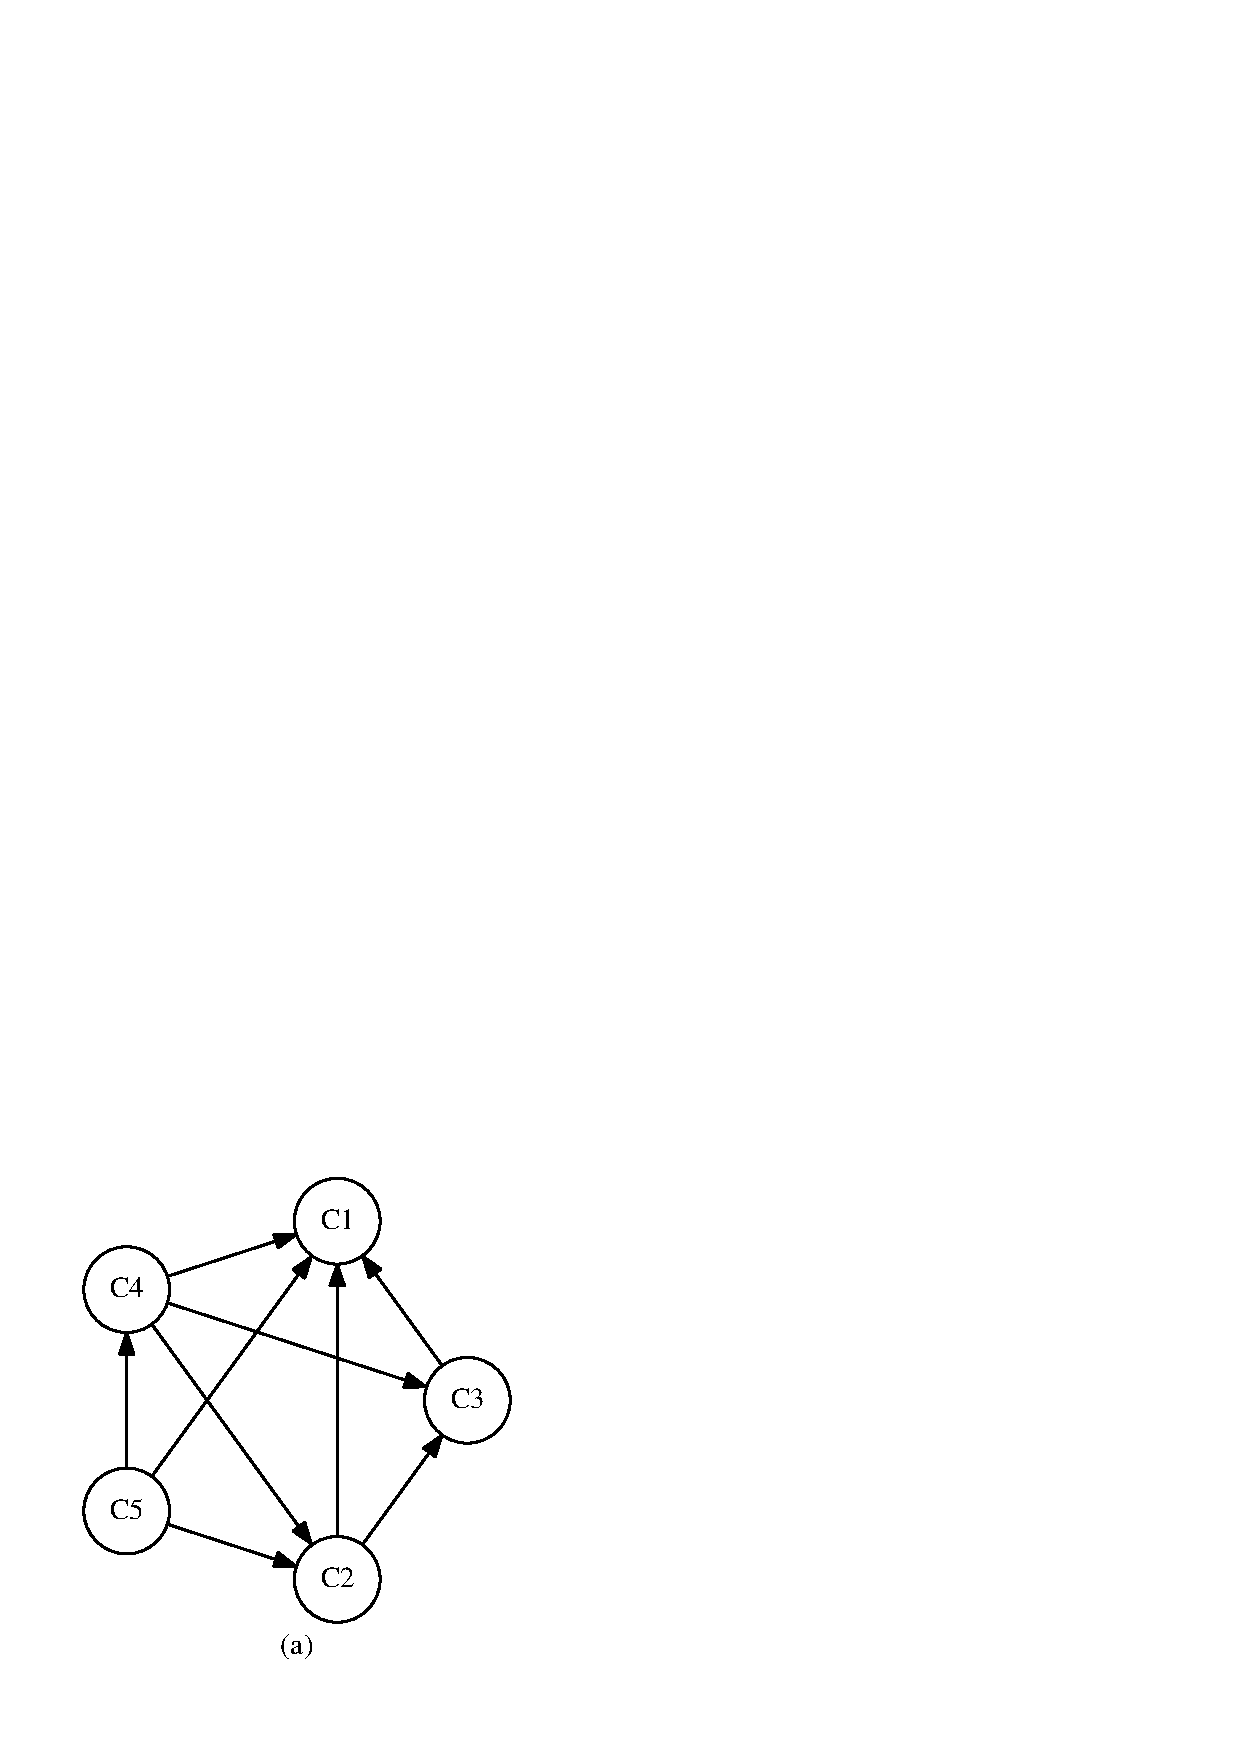
\includegraphics[width=0.42\columnwidth]{graphs/cart.pdf}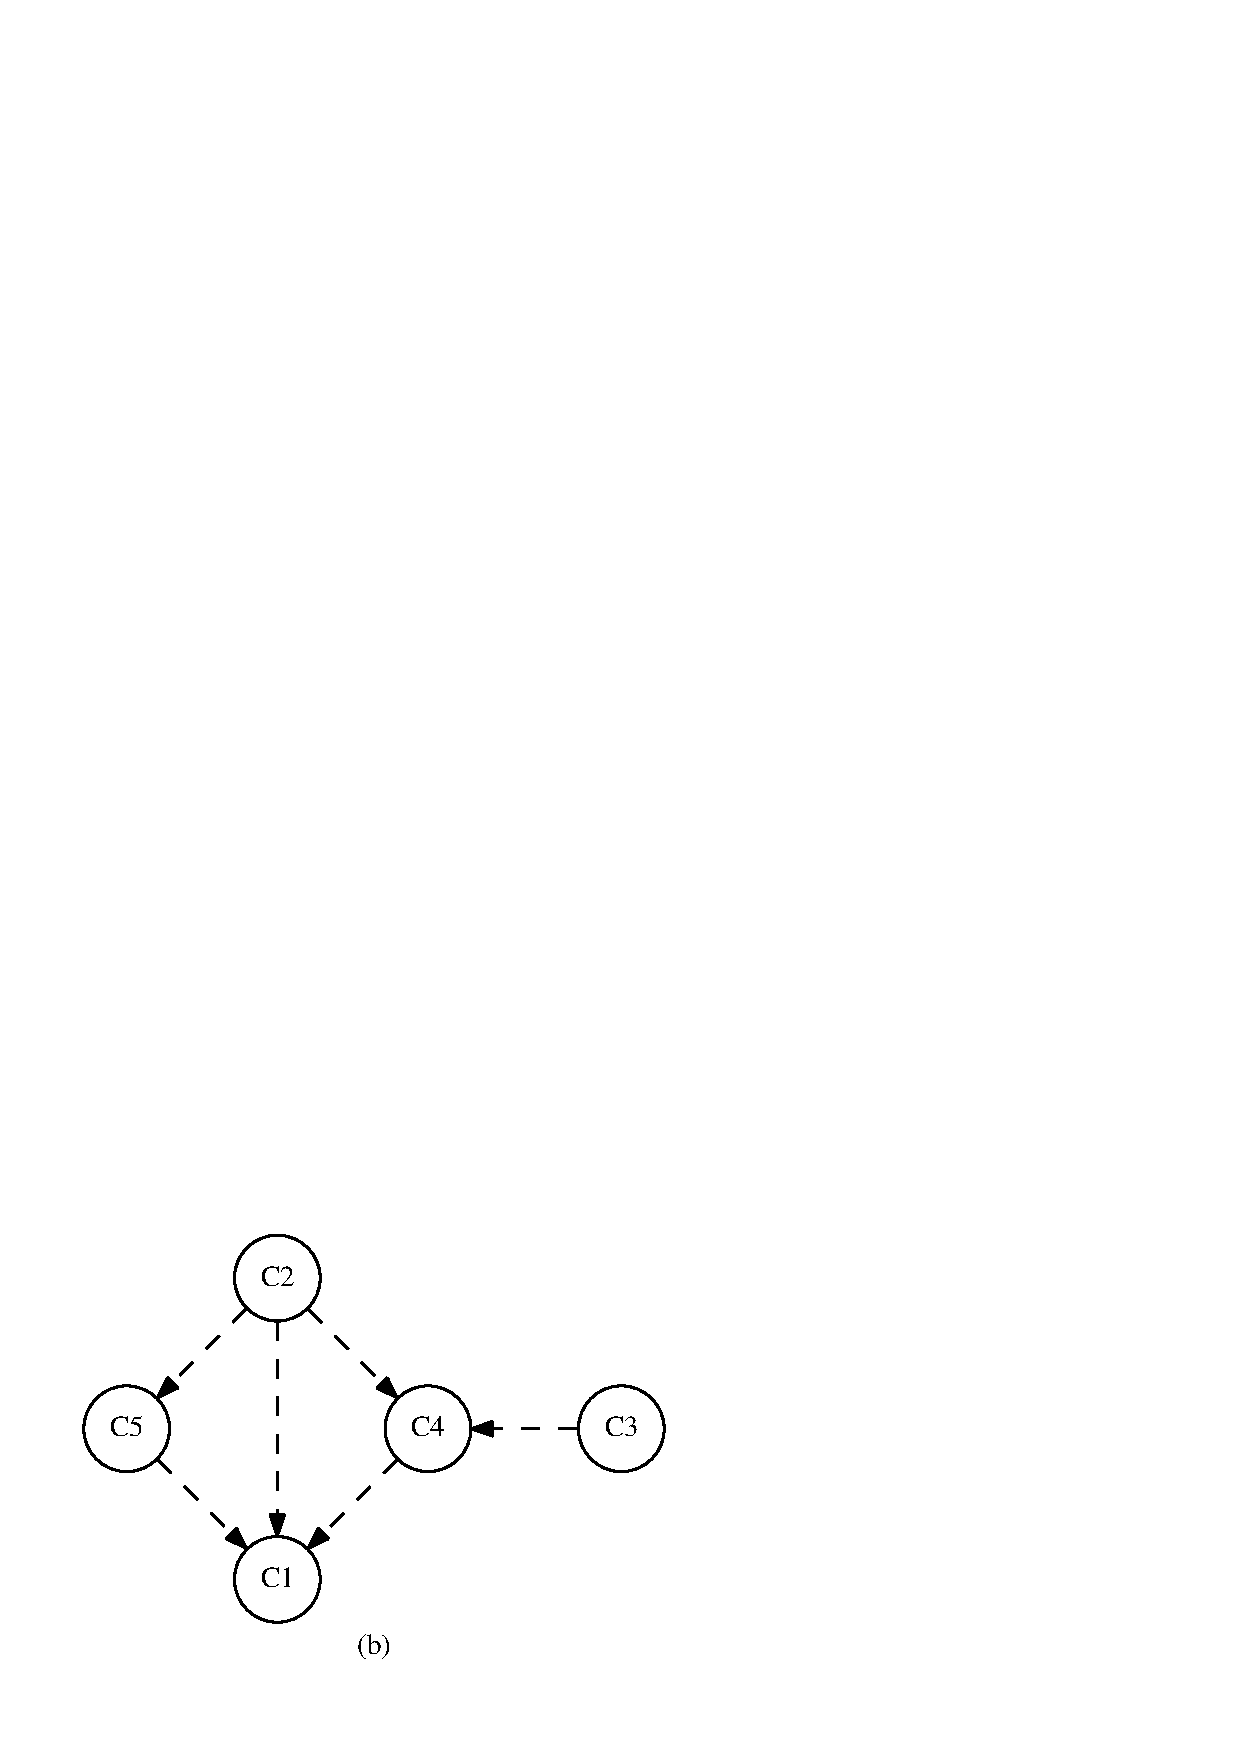
\includegraphics[width=0.57\columnwidth]{graphs/ccom.pdf}
\caption{Trend graphs for the CCC equivalence graph. Solid lines represent the artifact analysis. Dashed lines represent the understandability analysis.}
\label{fig:graphsforanalysis}
\end{figure}

\subsubsection{Building the Graphs}
In the community standards graph, we represent a directed edge from $C2 \rightarrow C1$ when  nPatterns(C1) $>$ nPatterns(C2) \emph{and}  nProjects(C1) $>$ nProjects(C2).
When there is a conflict between nPatterns and nProjects, as is the case between L2 and L3 where L2 is found in more patterns and L3 is found in more projects, an undirected edge is used.
This is to represent that there was no clear winner based on the two metrics used in the community standards analysis.
After considering all pairs of nodes in each equivalence class that also have an edge in Figure~\ref{fig:refactoringTree}, we have created a graph, for example Figure~\ref{fig:graphsforanalysis}a, that represents the frequency trends among the community artifacts. Note that with the CCC group, there is no edge between C3 and C5 because there is no straightforward refactoring between those representations, as discussed in Section~\ref{sec:refactoring}.

In the understandability graph, we represent a directed edge from $C2 \rightarrow C1$ when match(C1) $>$ match(C2) \emph{and} compose(C1) $>$ compose(C2). When there is a conflict between match and compose, as is the case with T1 and T3 where match(T1) is higher but compose(T3) is higher, an undirected edge is used. When one metric has a tie, as is the case with compose(C1) = compose(C5), we resort to the matching to provide the direction, in this case, C5 $\rightarrow$ C1. An example understandability graph is provided in Figure~\ref{fig:graphsforanalysis}b with the dashed arrows.
%\footnote{When there are confounded representations, as is the case with E8, E4, and E5 which all use tranformations from the CCC and the LIT equivalence classes, we omit those from the understandability graph. This makes sense since all use a transformation between T1 and T4 strongly favoring T1. }

\subsubsection{Topological Sorting}
Once the graphs are built for each equivalence class and each set of metrics, community standards and understandability, we apply a modified version of Kahn's topological sorting algorithm to obtain a total ordering on the nodes, as shown in Algorithm~\ref{topological}. In Kahn's algorithm, all nodes without incoming edges are added to a set $S$ (Line~\ref{addnoincomingtos}), which represents the order in which nodes are explored in the graph. For each $n$ node in $S$ (Line~\ref{beginwhile}), all edges from $n$ are removed and $n$ is added to the topologically sorted list $L$ (Line~\ref{addntoL}). If there exists a node $m$ that has no incoming edges, it is added to $S$.  In the end, $L$ is a topologically sorted list.

\begin{algorithm}
  \caption{Modified Topological Sort}\label{topological}
  \begin{algorithmic}[1]
\State  $L \gets$ []
\State $S \gets$ []
\State Remove all undirected edges (creates a DAG)
\State Add all disconnected nodes to $L$ and remove from graph. If there are more than one, mark the tie. \label{markTie1}
\State Add all nodes with no incoming edges to $S$. If there are more than one, mark the tie. \label{addnoincomingtos}
\While {$S$ is non-empty} \label{beginwhile}
	\State remove a node $n$ from $S$ \label{setn}
	\State add $n$ to $L$  \label{addntoL}
	\For {node $m$ such that $e$ is an edge from $n \rightarrow m$}
		\State remove $e$
		\If{$m$ has no incoming edges}
			\State add $m$ to $S$ \label{addToS}
		\EndIf
	\EndFor
	\State remove $n$ from graph
	\State If multiple nodes were added to $S$ in this iteration, mark those as a tie \label{markTie2}
\EndWhile
\State For all ties in $L$, use a tiebreaker.
  \end{algorithmic}
\end{algorithm}

One downside to Kahn's algorithm is that the total ordering is not unique. Thus, we mark ties in order to identify when a tiebreaker is needed to enforce a total ordering on the nodes. For example, on the understandability graph in Figure~\ref{fig:graphsforanalysis}b, there is a tie between C3 and C2 since both have no incoming edges, so they are marked as a tie on Line~\ref{markTie1}. Further, when $n=C2$ on line~\ref{setn}, both C5 and C4 are added to $S$ on Line~\ref{addToS}, thus the tie between them is parked on line~\ref{markTie2}. In these cases, a tiebreaker is needed.

Breaking ties on the community standards graph comes down to choosing the representation that appears in a larger number of projects, since it is more widespread across the community. Breaking ties in the understandability graph is trickier. Using Table~\ref{table:testedEdgesTable}, we compute the average matching score for all instances of each representation, and do the same for the composition score. For example, C4 appears in \todoLast{C2 -- C4}, \todoLast{C1 -- C4} and \todoLast{C3 -- C4} with an overall average matching score of 0.81 and composition score of 24.3. C5 appears in \todoLast{C1 -- C5} and \todoLast{C2 -- C5} with an average matching of 0.87 and composition of 28.28. Thus, C5 is favored to C4 and appears higher in the sorting.

\subsection{Results}
After running the topological sort in Algorithm~\ref{topological}, we have a total ordering on nodes for each graph. After breaking ties as described, the topological sorts for all graphs are shown in Table~\ref{topologicalResults}.  For example, given the graphs in Figure~\ref{fig:graphsforanalysis}a and Figure~\ref{fig:graphsforanalysis}b, the topological sorts are {\tt C1 C3 C2 C4 C5} and {\tt C1 C5 C4 C2 C3}, respectively.

\begin{table*}
\centering
\caption{Topological Sorting, with the left-most position being highest \label{topologicalResults}}
\begin{tabular}{|| l || l || l || l || l || l ||}
				& CCC			& DBB 		& LBW & SNG & LIT \\ \hline
Community Standards		& C1 C3 C2 C4 C5 	& D2 D1 D3	&  L3 L2 L1 	& S2 S1 S3 	& T1 T3 T2 T4 \\
Understandability 			& C1 C5 C4 C2 C3 	& D3 D1 D2 	& L3 L2		& S2 S1		& T1 T2 T4 T3 \\
\end{tabular}
\end{table*}




There is a clear winner in each equivalence class, with the exception of DBB.
That is, the node sorted highest in the topological sorts for both the community standards and understandability analyses are C1 for CCC, L3 for LBW, S2 for SNG, and T1 for LIT.
After the top rank, it is not clear who the second place winner is in any of the classes, however, having a consistent and clear winner is evidence of a preference with respect to community standards and understandability.

This positive result, that the most popular representation in the corpus is also the most understandable, makes sense as people may be more likely to understand things that are familiar or well documented. However, while L3 is the winner for the LBW group, we note that L2 appears in slightly more patterns.

CCC and DBB are shuffled quite differently, and LBW and SNG don't have enough information from the understandability analysis since there is just one edge. DBB is an odd one as the orderings are completely reversed depending on the analysis.


